\documentclass[12pt]{article}

\input preamble

\title{Principles of Parallel Architecture\\
Homework 1: Parallel Benchmarks}
\author{Xitong Liu \\
xliu@ece.udel.edu}

\begin{document}

\maketitle

\section{Question 1}
\begin{enumerate}

\item
\begin{description}
\item[Q: ]According to what the performance is measured? How often the 
rank is updated?
\item[A:]The performance is measured by their performance on the LINPACK 
Benchmark. The rank is updated twice a year.
\end{description}

\item
\begin{description}
\item[Q: ]Plot the performance of the fastest supercomputer vs time since 
1993. What can you comment on this plot?
\item[A: ]According to Fig.\ref{fig:fatest}, 
\begin{figure}[h!]
	\begin{center}
		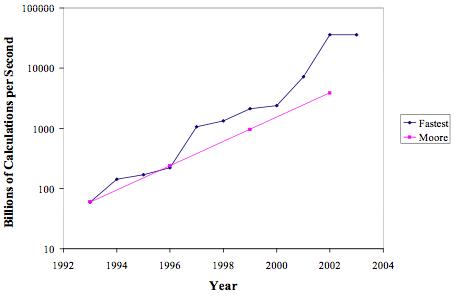
\includegraphics[width=0.7\textwidth, angle=0]{fatest.png}
		\caption{\label{fig:fatest}Fatest SuperComputer in the world}
	\end{center}
\end{figure}
the computing speed doubled roughly every 18 months, following 
the \textbf{Moore's Law}.
\end{description}

\end{enumerate}

\end{document}